\documentclass[12pt]{article}

\usepackage{apacite}
\usepackage[longnamesfirst]{natbib}
\usepackage{geometry} %for setting up margins
\usepackage{url} %this package lets a url appear in the bibliography
\usepackage[english]{babel}
\usepackage[autostyle, english = american]{csquotes}
\MakeOuterQuote{"}  % the previous lines make it so that the quotation marks all appear the right way around 

\usepackage{tabto}
%\usepackage{listings} %for inserting R scripts
%\usepackage{verbatimbox}

\usepackage{fancyvrb} %centre verbatim box

%for the figure stuff
\usepackage{subfig}
\usepackage{wrapfig}
%\usepackage{subfigure}
%\usepackage{subcaption}
\usepackage[justification=centering]{caption}
\usepackage[bottom]{footmisc}
% to set up the figures to be apa
%\captionsetup[figure]{labelsep=period,labelfont=it,justification=justified,singlelinecheck=false,font=doublespacing}
% add in font=doublespacing

\usepackage{fancyhdr} %Just used to make nice headers and footers 


\pagestyle{fancy}
\fancyhf{}
\fancyhead[LE,RO]{Penguins are cooler than you}
\fancyfoot[LE,LO]{Page \thepage}

\renewcommand{\headrulewidth}{2pt}
\renewcommand{\footrulewidth}{1pt}

\usepackage{graphicx}


\usepackage[normalem]{ulem} %this adds the \uline{} function which stops underlined titles from running off the page 
\usepackage{hyperref} % This package makes it so that your citations become hyperlinks to the web url provided or to the reference section... That's really cool [colorlinks=true,linkcolor=blue,citecolor=blue]

\geometry{a4paper, total={170mm,257mm}, left=20mm, top=20mm}
\usepackage{setspace}
\linespread{1.5} %says there's a problem but it seems to work for line spacing




\begin{document}

\begin{titlepage}
	\centering
	{\huge\bfseries Penguins are cool\par}
	\vspace{1cm}
	Warren \textsc{James}, \par
	Dr.~Josephine \textsc{Reuther}, \par
	Ellen \textsc{Angus}, \par
	Dr.~Amelia \textsc{Hunt},\par
	and\par
	Dr.~Alasdair \textsc{Clarke}
	\vfill
\end{titlepage}	


\newpage

%% ABSTRACT
\begin{center}
	\section*{Abstract}
\end{center}

\begingroup\singlespacing
\newpage
\tableofcontents
\newpage
\endgroup

%% Itroduction
\section*{Introduction}
\addcontentsline{toc}{section}{Introduction}
\paragraph{} Everyday we make use of our visual system in order to solve many problems. Whether these are to aid us in avoiding obstacles, or to find an item of importance, the ability to direct our attention proves invaluable. However, the extent to which we make these decisions in an optimal manner is subject to debate. 

\paragraph{} \cite{najemnik2005optimal} argue that human performance in a visual search task is predicted by that of a model ideal observer. This model aimed to reduce uncertainty as to the location of a target item by deploying fixations to locations likely to contain the target and reduce the overall uncertainty of the search space. To do this, the model accounted for the loss of accuity for space further from the central fixation and using this information to reduce the amount of uncertainty to an appropriate extent. This in turn aids in finding a target as it would help in dissuading us from revisiting a location that we have already searched to an appropriate extent. 

\paragraph{} This would suggest that we make decisions about where to fixate based on underlying scene statistics and account for our own limitations. However, this would seem to be a fairly resource intense process which begs the question as to whether this would be an appropriate solution to the problem of where to fixate. With this in mind, \cite{clarke2016stocha} suggest that human performance in a visual search task can be characterised by a stochastic process. Instead of engaing in a resource intense calculation of where to fixate, they suggest that we make eye movements that we like to make in a more stochastic process. 

\paragraph{} As such, this leaves us with the question of whether we make principled fixations based on various factors, or whether we simply do what we like to do and fixate locations in a more random fashion. One way in which this question could be addressed is by simplay tasking people with making one sensible eye movement. If we fixate based on principle, then to complete a task such as this should prove to be trivial. 

\paragraph{} Much to the contrary it appears that people do in fact tend to struggle at making one sensible eye movement \citep{morvan2012human,clarke2015failure}. \cite{morvan2012human} developed a paradigm in which participants were to make a single eye movement in order to give themselves the best chance of success at detecting whether a target dot was positioned at the top or the bottom of a box \textbf{\textit{(point to figure when you have one?)}}. To do this, three boxes were presented on screen. One in the centre, with two boxes either side. Participants were told that they were to fixate one of these boxes and that the target would then appear in one of the two side boxes. Throughout the experiment, these two side boxes would appear at difference eccentricities, sometimes being placed very close to the centre box, and at other times they would be a large distance from the central box. When the boxes were all close together, the optimal strategy would be to fixate the central box and use one's peripheral vision to detect the target. However, as the boxes separated, performance would begin to decrease. In this case, participants engaging in the optimal strategy would switch to focussing one of the two side boxes as this would then give them the best chance of success. 

\paragraph{} The results of their experiment clearly demonstrated that people failed to perform this task in an optimal fashion. These results were further supported by \cite{clarke2015failure} who replicated this study with the addition of including other versions of the task that were not specific to eye movements. This would suggest that this failure is not constrained to optimal search, but more a general failure to maximise the chance of success. 

\section*{Methods}
\addcontentsline{toc}{section}{Methods}

\subsection*{Participants}
\addcontentsline{toc}{subsection}{Participants}
\paragraph{} Participants were recruited via word of mouth at the University of Aberdeen. In total, 18 participants took part in the experiment (13 female) with an age range of 20-23 (mean of 20). 

\subsection*{Procedure}
\addcontentsline{toc}{subsection}{Procedure}
\paragraph{} The experiment took part over two sessions. The first session was to measure each participant's visual acuity in order to tailor the second session to each individual. The first session lasted approximately 30 minutes. In the second session, participants carried out the actual decision task, which lasted between 40 and 50 minutes. 

\paragraph{} Both sessions made use of and Eyelink 1000 (version 4.594) (SR Research ltd, Mississauga, Ontario, Canada) which recorded eye position at 1000 Hz. Participants were sat $\approx45cm$ from the screen, which was maintained throughout the experiment by use of an adjustable chin rest. \textit{Was this experiment on the OLED?}. The experiment was programmed and run in Matlab 7.9.0 (R2009b) with Psychtoolbox \citep{pelli1997videotoolbox} and EyelinkToolbox functions \citep{cornelissen2002eyelink}. Prior to starting each session, a 5-point calibration was carried out. Participants were recalibrated prior to starting a new block. Additionally, they were also recalibrated if they had failed to fixate appropriately 10 times since the last calibration, or if there were 5 errors in a row.

\subsubsection*{Session 1}
\paragraph{} In the first session, participants were presented with a fixation cross with two boxes placed either side \textit{\textbf{get fig}}. They were told that their task was to identify whether a small dot \textit{\textbf{get size of this dot}} had appeared in the top or the bottom half of one of the boxes (each $\approx1^{\circ}$). It did not matter which box it had appeared in, they were simply to report whether it was up or down by pressing the "up" or "down" arrow, respectively, on the keyboard. To commence each trial, participants had to press the space bar whilst fixating the central cross. After maintaining fixation for 700ms, the target dot would appear in one of the two boxes, at random, and was displayed for 700ms (\textit{\textbf{Need to double check all this}}). If participants broke fixation during any stage of this process, the screen would turn red for 700ms to indicate that they had broken fixation. 

\paragraph{} The boxes were presented at varying separations from the central fixation cross ($2.7^{\circ}$, $3.9^{\circ}$, $5.2^{\circ}$, $6.8^{\circ}$, $8.4^{\circ}$, $10.1^{\circ}$, $11.4^{\circ}$, $12.5^{\circ}$). There were 4 blocks in total, with each different separation being presenter 12 times in a pseudo-random order. This meant participants completed 4 blocks of 96 trials. Data from this session was then used to work out the point at which participants were 75\% accurate in detecting the target. This value was then used in the second session to tailor the experiment for each individual.

\subsubsection*{Session 2}  
\paragraph{} For the second session, participants were introduced to "\textit{Pugadoo}". They were told that there task was to help Pugado collect as many fish as possible. In order to do this, they would be choosing a box to fixate in order to detect whether the target dot was in the upper or lower half of one of the two side boxes (\textit{\textbf{Get fig}}). On each trial, participants would see Pugadoo and have to fixate the star on their stomach to start the trial. They would then press the space bar and three boxes would appear. Participants were told they could fixate any one of the three boxes but that the target would only ever appear in one of the two side boxes at random. These boxes were placed at various distances from the centrally presented box. These distances were defined in relation to the switch point that was calculated based on their performance in the first session. Seven were defined as the switch point in the following way; switch point $-3^{\circ}$, $-2^{\circ}$, $-1^{\circ}$, $0^{\circ}$, $+1^{\circ}$, $+2^{\circ}$, $+3^{\circ}$. A further two distances were added so as to be constants across all participants ($8^{\circ}$ and $18^{\circ}$). 

\paragraph{} For every trial that the participants correctly identified the position of the target dot, the background would turn green and the bar in the top left corner would fill by one tick. After having filled the bar to the top, Pugadoo would be rewarded with a fish and the bar would return to being halfway filled. If the participant was incorrect, the background would turn red and the bar would be emptied by one tick on the bar. If the bar was fully depleted, a fish would be taken away from the total. This allowed participants to monitor their performance while completing the task. 

\paragraph{}

\section*{Results}
\addcontentsline{toc}{section}{Results}
\paragraph{} All analysis was carried out in R version 3.4.3 \citep{R} using Rstan \citep{Rstan,Stan}. Additional data was retrieved from \url{https://osf.io/t6c5q/} in order to compare the current study's data to a group without the presence of a clear goal, but who otherwise carried out the same task. The full methods and analysis of this comparison data can be found by following the link provided. 

\paragraph{} For the purposes of this study, the first four blocks completed by participants in this comparison set were used. In the firsr four blocks of this other study, particiapnts either carried out the standard task as described in \cite{clarke2015failure}, or they were effectively instructed as to where they should fixate on each trial in order to achieve the optimal accuracy (henceforth referred to as the "\textit{control}", and the "\textit{optimal}" group respectively).

\subsection*{Fixation Proportions}
\paragraph{} On each trial, participants were given three possible locations to fixate. Fixations were coded as being either a central fixation (i.e., they fixated the centre box), or as a side fixation (i.e., they fixated one of the side boxes). A proportion was then calculated for how often the participant fixated one of the side boxes within each of the distances mentioned in the methods section. 

\paragraph{} From an intial inspection of Figure \ref{fig:Position_raw}, participants in the motivated group do not appear to be doing anything different to those in the Control group. They certainly do not look as though they have been instructed as to where to look if one compares their results to the Optimal group. 

\paragraph{} \textit{I do have model results for this... but I imagine this can be added to the supplementary material? Also, it's pretty uniformative as to what's happening and doesn't add more to what can already be seen in the figure anyway}

\begin{figure}[ht!]
	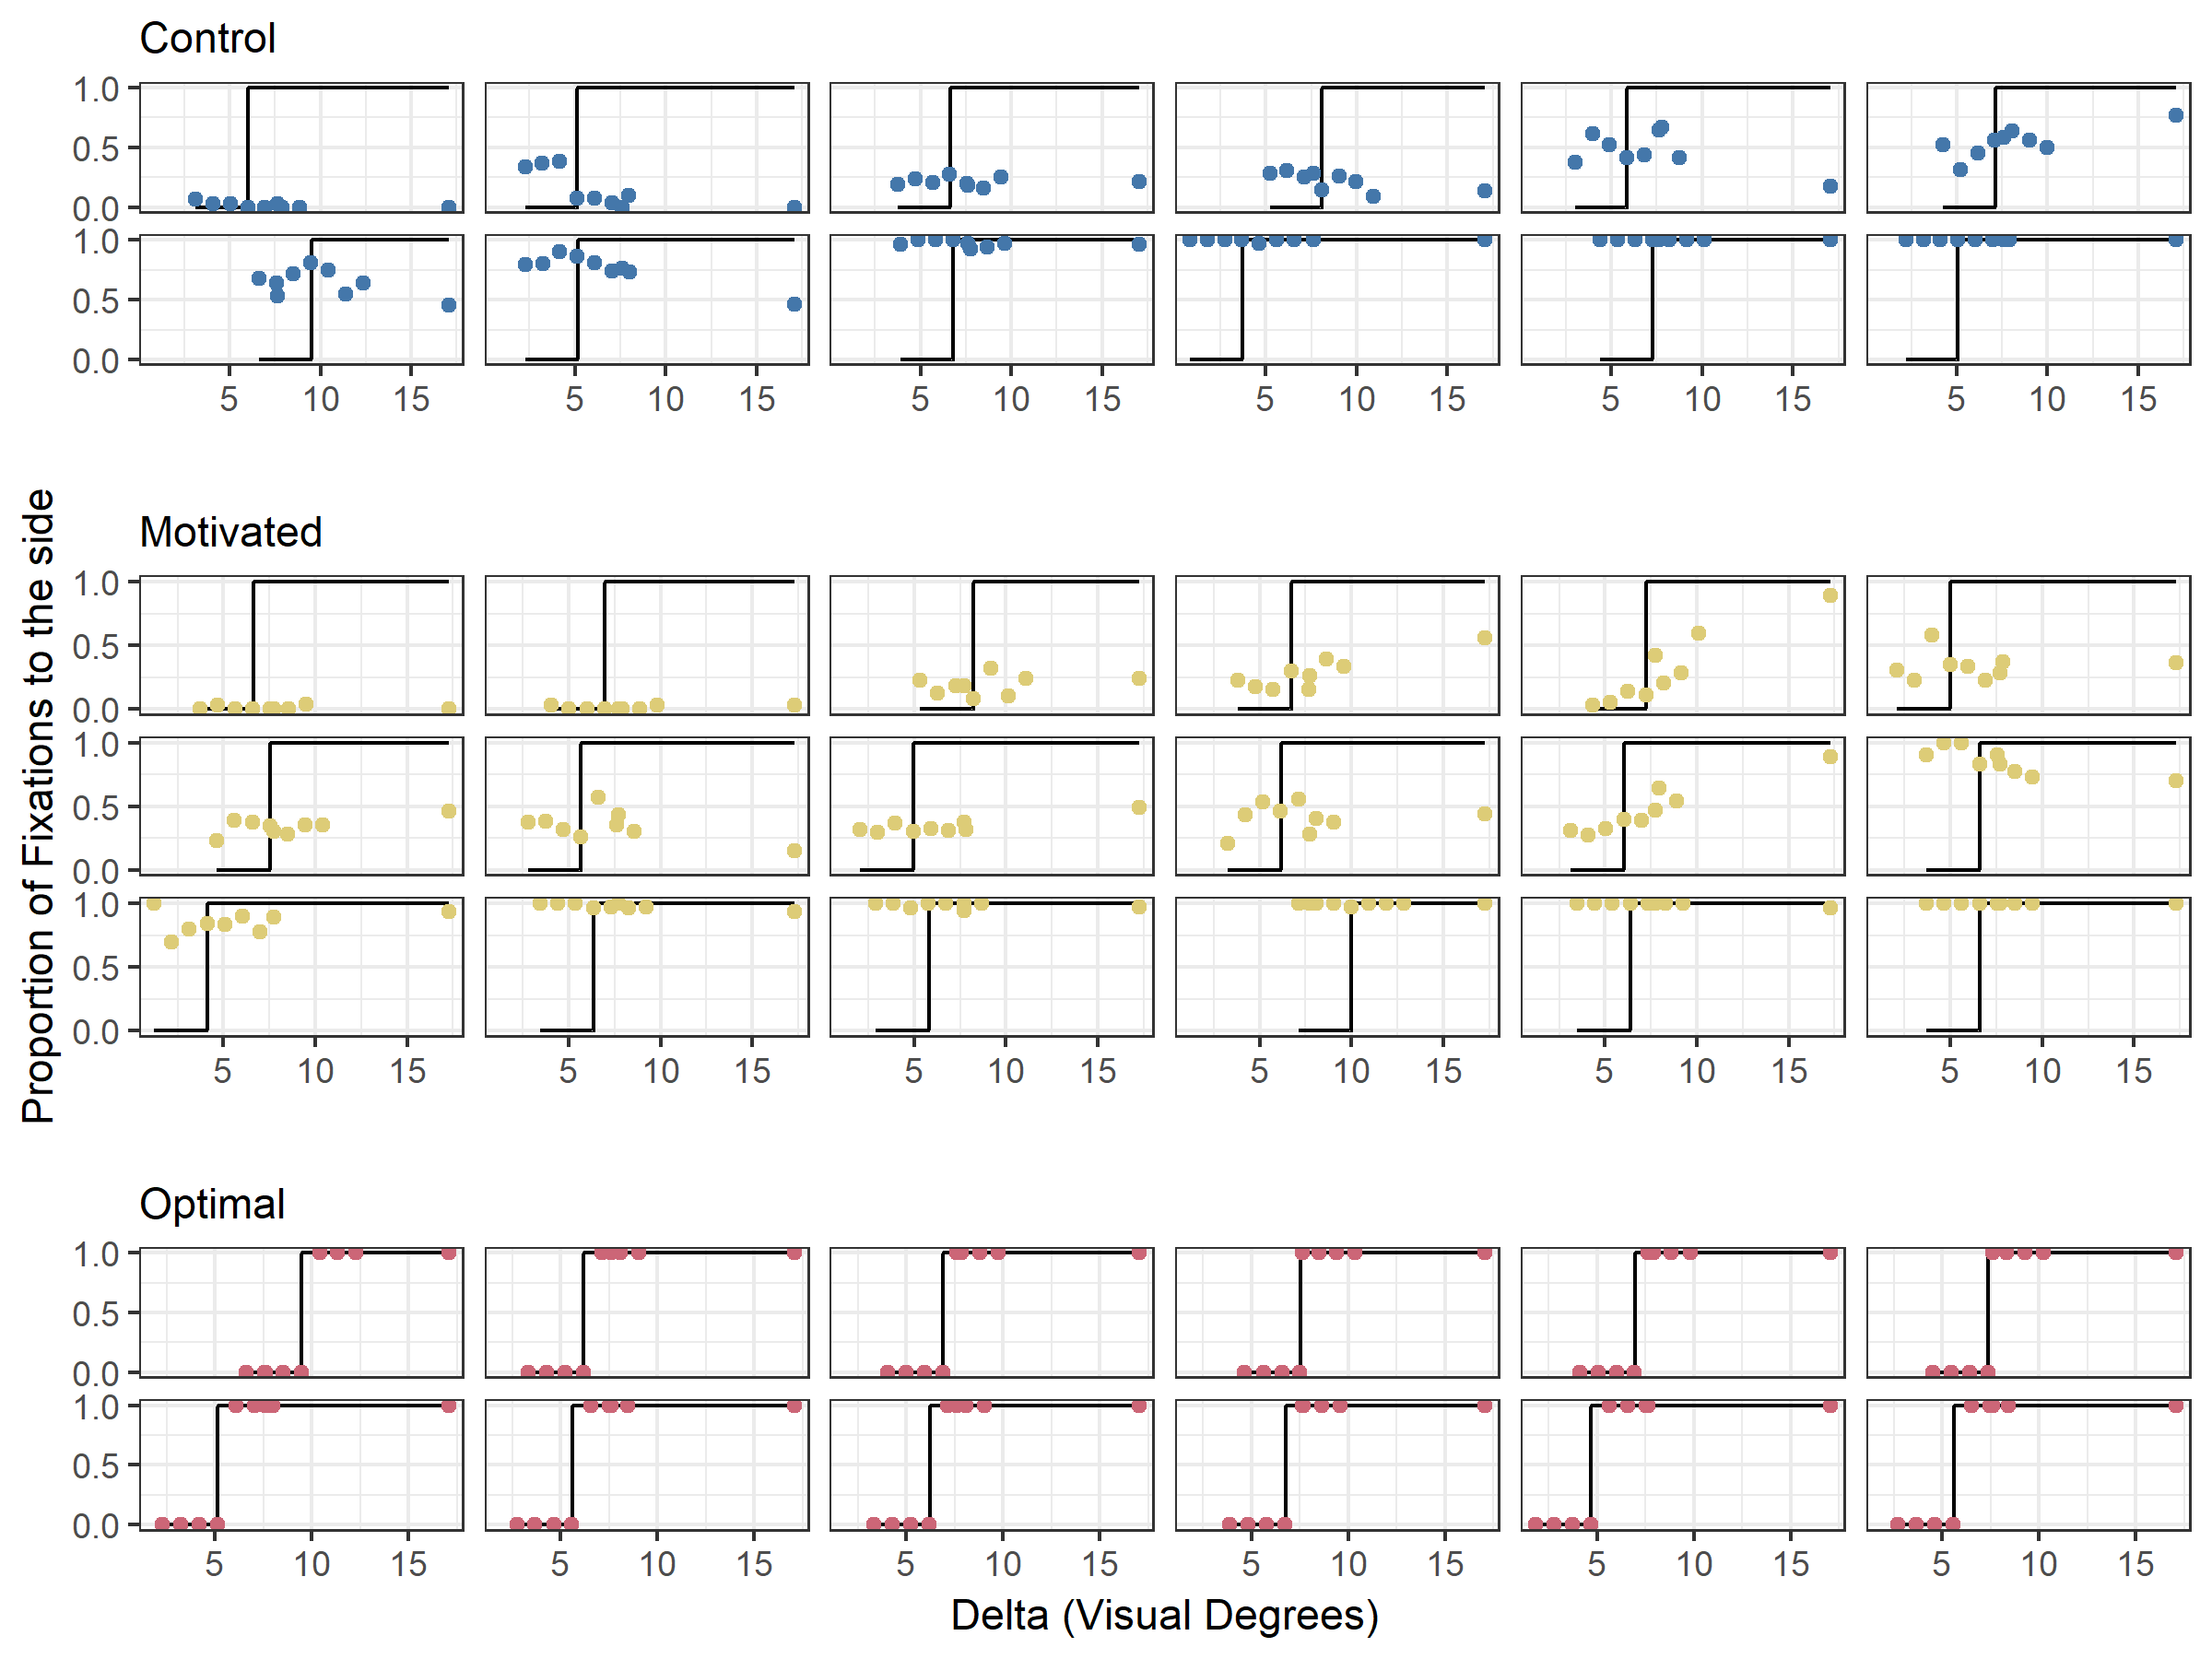
\includegraphics[scale=0.7]{../Figures/Part_2_all_groups.png}
	\centering
	\captionsetup{justification=centering}
	\caption{Plot of proportion of fixations to the side box (y-axis) with increasing Delta (x-axis). The bottom set of plots (in red) demonstrate what behaviour would look like if participants had employed an optimal fixation strategy}
	\label{fig:Position_raw}
\end{figure}

\subsection*{Rate of Success} 
\paragraph{} Initial analysis for rate of success examined overall accuracy for each pariticipant. To do this, an average was calculated for each participant which was then modelled using a Bayesian Regression Model with a Beta family. All priors were left as uniform and therefore uniformative. Rate of success was modelled using group as a predicor variable. Delta was not investigated as we are first and foremost interested in the participant's overall rate of success. 

\paragraph{} \textit{Should the analysis that included Delta be presented in the supplementary material? Pretty sure it does help with the model fit, but it's not entirely necessary for the conclusions of this paper?}

\begin{figure}[ht!]
	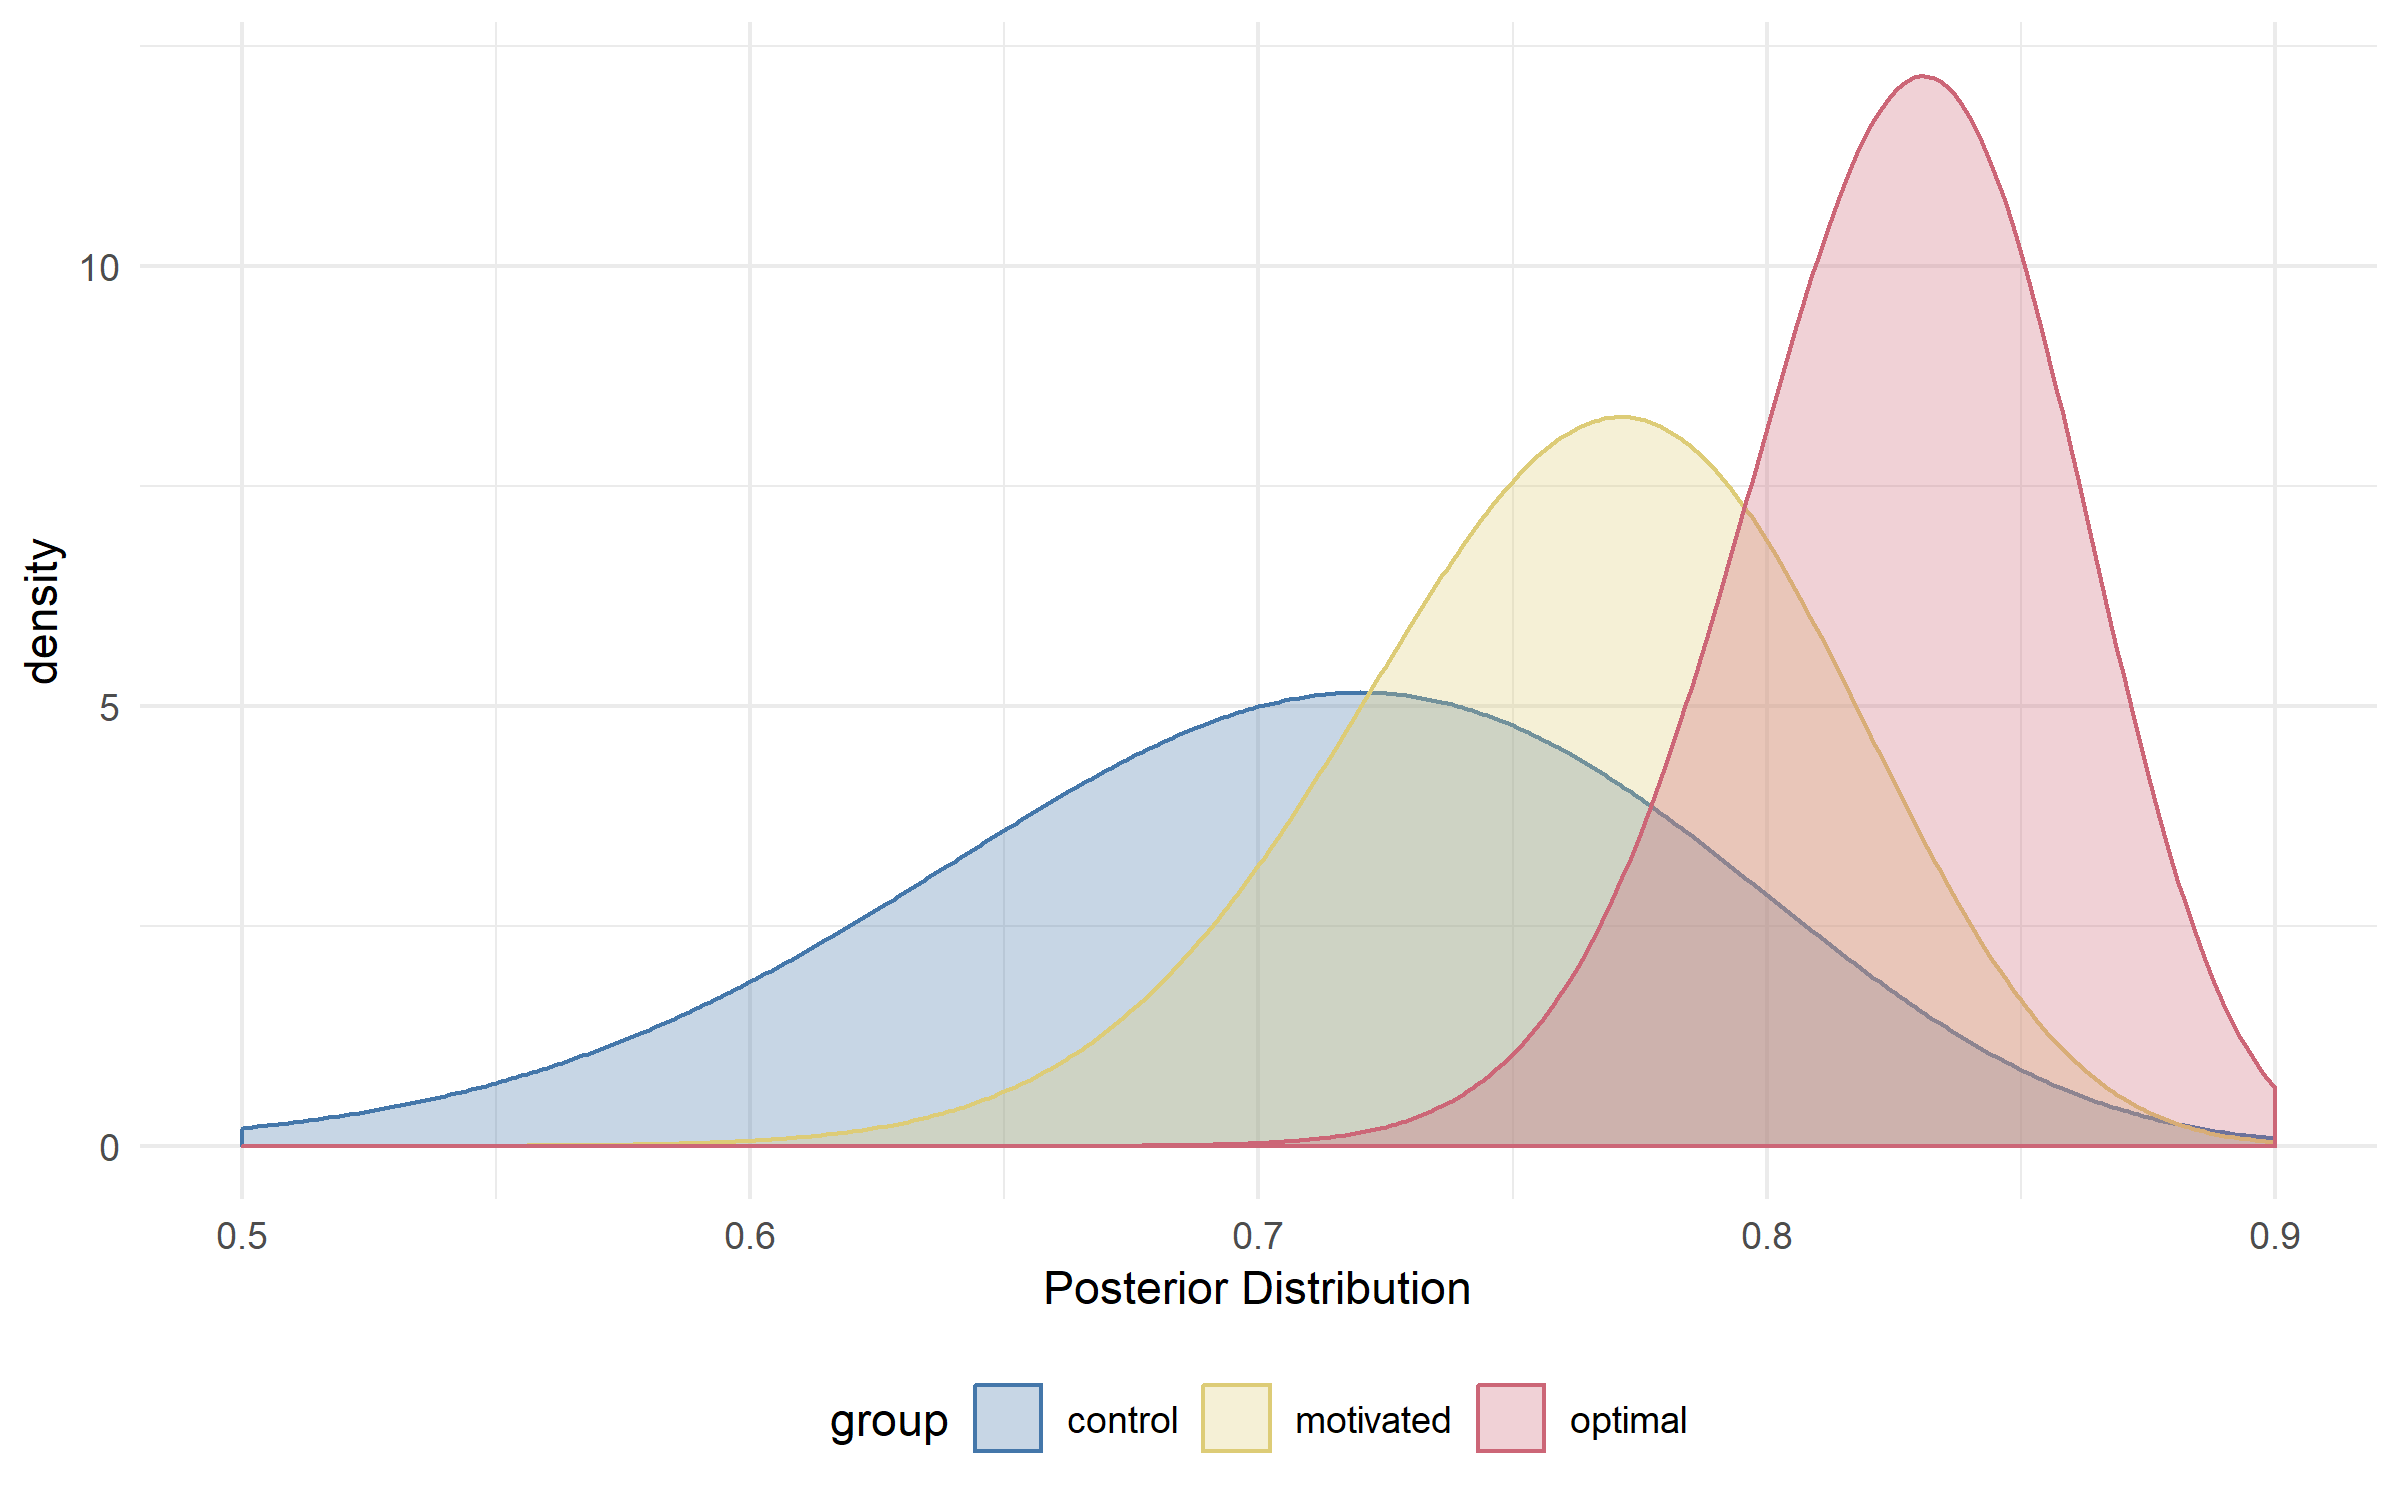
\includegraphics[scale=0.8]{../Figures/Model_stan_rawacc.png}
	\centering
	\captionsetup{justification=centering}
	\caption{Posterior predictions for raw accuracy.}
	\label{fig:Model_raw_acc}
\end{figure}

\paragraph{} In Figure \ref{fig:Model_raw_acc}, it can bee seen that that the Motivated group were generally more successful than the Control group. The Control group had a predicted mean rate of success of $0.708$ with a 95\% HPDI of $|0.661, 0.747|$, and the Motivated group had a mean of $0.764$ with a 95\% HPDI of $|0.74, 0.789|$. However they did not reach the same level of success as the optimal group which had a mean success rate of $0.825$ with a 95\% HPDI of $|0.805, 0.844|$. 

\paragraph{} This result seems somewhat surprising given the fixation proportions that can be observed in Figure \ref{fig:Position_raw}. As such, additional analyses were carried out.

\subsection*{Expected Rate of Success}
\paragraph{} In order to make a fairer comparison of the groups, each participant's expected success rate was calculated given the fixations choices they had made on each trial. For example, if the boxes were far apart and the participant had fixated one of the side boxes on that trial, they would have a $\approx$100\% chance of success at the fixated box (b$_f$) and $\approx$50\% chance of success at the non-fixated box (b$_{nf}$) as this would be imperceptable but they would have a 50\% ($c$) chance due to the nature of the task. Each of these boxes would be equally likely to contain the target and so the expected chance of success on a trial like this would be 75\% which is given by calculating $(b_f + b_{nf})\times c$. This was calculated for each participant, on each trial. This was then averaged for each participant to give an average expected accuracy. 

\paragraph{} After accounting for chance, the difference that was once observed when modelling participant's raw success rate (Figure \ref{fig:Model_raw_acc}) appeared to entirely dissapear. Inspecting Figure \ref{fig:Model_exp_acc} would demonstrate that participants in the Motivated (mean of $0.735$, 95\% HPDI of $|0.715, 0.754|$) and Control (mean of $0.732$, 95\% HPDI of $|0.706, 0.755|$) groups almost identical expected success rates as can be seen by the almost entirely overlapping posterior predictions. These results would suggest that the previously greater rate of success experienced by the Motivated group was not due to them making better, strategical decisions about where to fixate. Instead, this greater rate of success would appear to be due to something other than a more optimal strategy being utilised. 


\begin{figure}[ht!]
	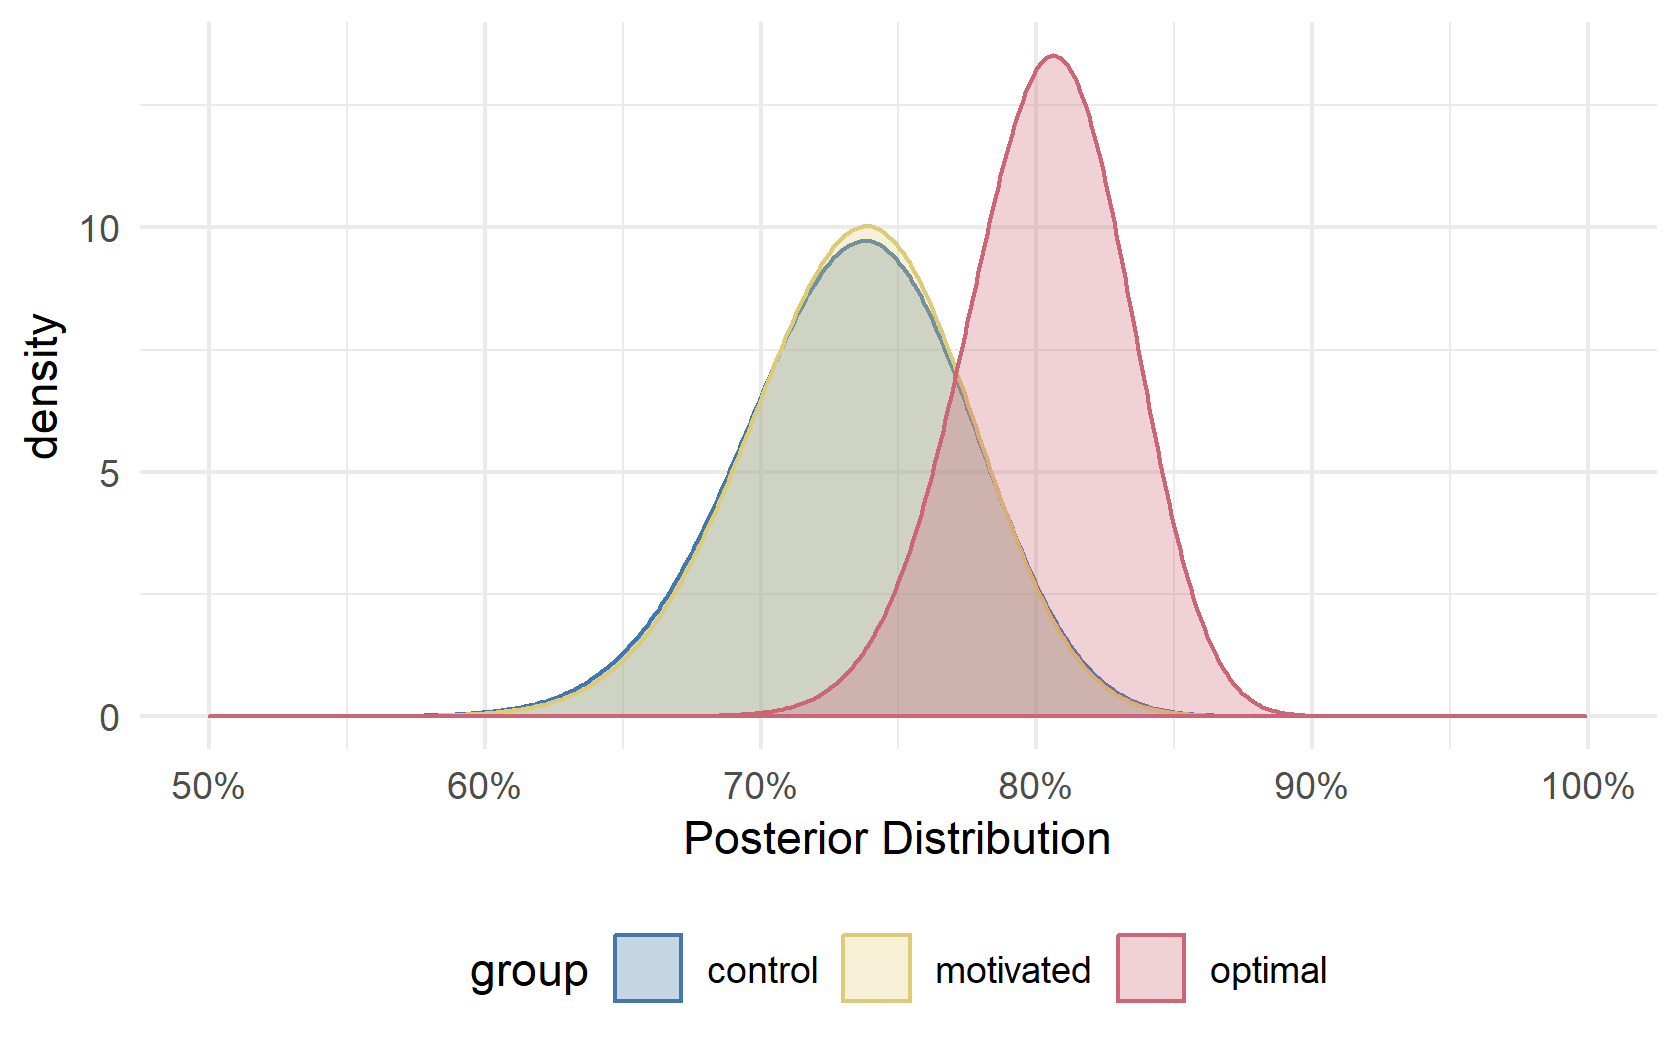
\includegraphics[scale=0.8]{../Figures/Model_stan_expacc.png}
	\centering
	\captionsetup{justification=centering}
	\caption{Model output for expected success rate.}
	\label{fig:Model_exp_acc}
\end{figure}

\section*{Discussion}
\addcontentsline{toc}{section}{Discussion}

\section*{Conclusion}
\addcontentsline{toc}{section}{Conclusion}

% Bibliography
\clearpage
\begingroup\onehalfspacing
\newpage
\addcontentsline{toc}{section}{References}
\bibliographystyle{apacite}
\bibliography{MD_bib}
\endgroup

\end{document}